\section{Background} \label{Background}

This section outlines the beginnings of blockchains applied in cryptocurrency systems like Bitcoin and Ethereum, and also describes the ByzCoin blockchain which was selected as most appropriate for this project.

\subsection{Bitcoin Blockchain} \label{Bitcoin}
The blockchain concept drew attention in 2008 when Satoshi Nakamoto introduced the Bitcoin \cite{Bitcoin} system for electronic transactions that rely on cryptographic primitives instead of trusting a third party. A brief description of the Bitcoin cryptocurrency system goes as follows:
\newline
Whenever Alice wants to transfer digital money ("coins") to Bob, she creates a transaction and broadcasts it to a peer-to-peer network. This transaction consists of a digital signature (using the private key of Alice) of the hash of the previous transaction related to these coins, together with the public key of the next owner - Bob \cite{Bitcoin}.
\newline
Hence, Bob has access to the chain of ownership of the coins he has received, but still does not have a proof that Alice has not sent the same coins to another person. This double-spending problem is solved by requesting the nodes of the peer-to-peer network to agree on a single order of transactions, so that only the earliest transaction counts \cite{Bitcoin}.
\begin{figure}[H]
    \centering
    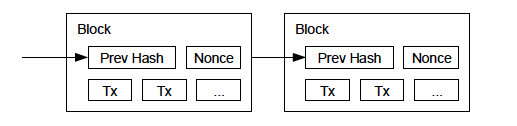
\includegraphics[width=1\textwidth]{Figures/blocks_bitcoin.png}
    \caption{Blocks in Bitcoin \cite{Bitcoin}}
    \label{Blocks in Bitcoin}
\end{figure}
\noindent
Every participant of the network needs to first verify that the transaction initiated by Alice does not use already spent digital money, and then place it together with other transactions in a block that is supposed to be added on a chain of blocks (Figure~\ref{Blocks in Bitcoin}). To save space, the transactions are hashed in a Merkle tree \cite{Merkle}, and only the root of the tree is included in the header of the block. In order to append a new block, the node, also called miner, needs to solve a computing difficult task called proof-of-work (PoW) that involves scanning for a value (nonce) that produces a hash which begins with a determined number of zero bits \cite{Bitcoin}. As input to the hash function, in addition to the nonce, there is also the hash value of the previous block. This way, by hashing the transactions into a chain, it is impossible for attackers to change a record without re-computing previous PoWs \cite{Bitcoin}.\\
\newline
It can happen that two or more participants find a proof-of-work at
nearly the same time, and this is going to create forks in the blockchain.
To solve this issue, only the longest branch of blocks and the transactions taking part of it is valid. Hence, the historical order of transactions is unique and the same for everyone.\\
\newline
A transaction in the Bitcoin blockchain is considered to be confirmed with high
probability only after six additional blocks have been appended behind it. The block mining rate is 10 minutes on average. This introduces high latency in the system and hinders real-time transactions (Imagine waiting one hour for a coffee you have bought with your digital coins). 
\newline
Some other inconveniences also exist like waste of resources caused by the unsuccessful miners when they are trying to append a new block. Furthermore, even though the Bitcoin blockchain documentation \cite{Bitcoin} ensures correct processing of transactions if the majority of computing power is not owned by malicious miners, there are still some vulnerabilities like strategic mining attacks \cite{Attacks1,Attacks2}.

\subsection{Ethereum Blockchain}

Since the Bitcoin cryptocurrency system created a revolution in the world of decentralized systems, many other blockchain protocols and applications started appearing, either to improve on Bitcoin or to find usage in other fields (e.g. health care \cite{Health}).\\
\newline
One of the nowadays best known blockchain protocols is Ethereum \cite{Ethereum}, due to a universality principle that allows users to create their own rules for state updates ("contracts") using internal scripting language and then apply these smart contracts in a variety of blockchain based applications (financial, semi-financial and not financial at all, like online voting and decentralized governance) \cite{Ethereum}.
\newline
The straightforward way of creating digital contracts that autonomously enforce the rules of interaction and are precompiled in the nodes that maintain the blockchain \cite{Ethereum}, is one of the most significant benefits one can get for choosing Ethereum over the Bitcoin blockchain protocol.\\
\newline
Ethereum can be interpreted as a transaction-based state machine where every new valid transaction leads to a state transition \cite{Ethereum}. Similarly, like in Bitcoin \cite{Bitcoin}, for appending a new block of transactions, a miner needs to perform a computationally difficult task, with the underlying algorithm Ethash, in order to find a proof-of-work before other competitors. An advantage of Ethash is that it is ASIC-resistant, meaning that finding a nonce requires a lot of memory
and it is not possible to use the same memory for discovering multiple nonces in parallel. Accordingly, this allows better decentralization by making the distribution model
as open as possible and preventing malicious miners to skew the
distribution in their favour \cite{Ethereum}.\\
\newline
Overall, Ethereum guarantees that every two individuals can be confident that the outcome of their interaction will be in coordination with the specified digital contract.

\subsection{ByzCoin Blockcain} \label{ByzCoin Background}

The proof-of-work technique utilized in the Bitcoin blockchain protocol \cite{Bitcoin}, solves the consensus problem - several processes deciding on one value from a set of proposed values (in this particular case: which update of the state of the distributed ledger to follow). However, it only provides probabilistic consistency guarantees, meaning that clients cannot immediately be certain that a submitted transaction is committed even though it has been added on the blockchain \cite{ByzCoin}. As mentioned in section~\ref{Bitcoin}, it takes at least one hour for a transaction to be considered confirmed with high probability.\\
\newline
The blockchain introduced by the EPFL DEDIS (Decentralized and Distributed Systems) Laboratory solves this transaction commit latency problem, by replacing Nakamoto's consensus \cite{Bitcoin} with a Practical Byzantine Fault Tolerance \cite{PBFT} based protocol called ByzCoinX \cite{OmniLedger}. An improvement on top of PBFT, that reduces the costs of the multiple rounds of this protocol, is the inclusion of CoSi \cite{CoSi} - a collective signing protocol that aggregates thousands of signatures \cite{ByzCoin}. 
ByzCoinX uses collective signing to achieve consensus with absolute finality property (transactions are irreversibly committed within seconds unlike with probabilistic finality), and at the same time preserves the open membership characteristic of a public ledger like Bitcoin \cite{ByzCoin}.
\newline
The servers that run the ByzCoinX protocol and offer decentralized services to users, are called collective authority nodes or later on referred to as co-nodes.\\
\newline
In this protocol, there is a leader which is responsible for contacting every other node in the system in order to collect transactions submitted by end users. For the communication, as well as for the collective signing, ByzCoinX uses a tree structure with the leader as root, which significantly reduces the transaction confirmation latency in the system \cite{ByzCoin}.
\newline
Once the leader receives transactions from the followers, a block containing the transactions is being created and sent back to the followers for validation. If there are remaining transactions, they will be considered upon creation of the next block \cite{ByzCoin Impl}.
\newline
In case the leader starts behaving maliciously or simply does not perform as expected, the followers initiate a \textbf{view change} (change of the leader) \cite{ByzCoin Impl}.\\
\newline
In a similar fashion like in Ethereum \cite{Ethereum}, the ByzCoin blockchain protocol works with smart contracts precompiled into the conode binary, that define how a certain instruction updates the global state.  The leader computes this state change, but every conode verifies whether it is correct. The global state consists of instances, each one of which is tied to a contract and holds data (Figure~\ref{ByzCoin}). A Merkle tree \cite{Merkle} root of the global state is stored in every header of a block.\\
\begin{figure}[H]
    \centering
    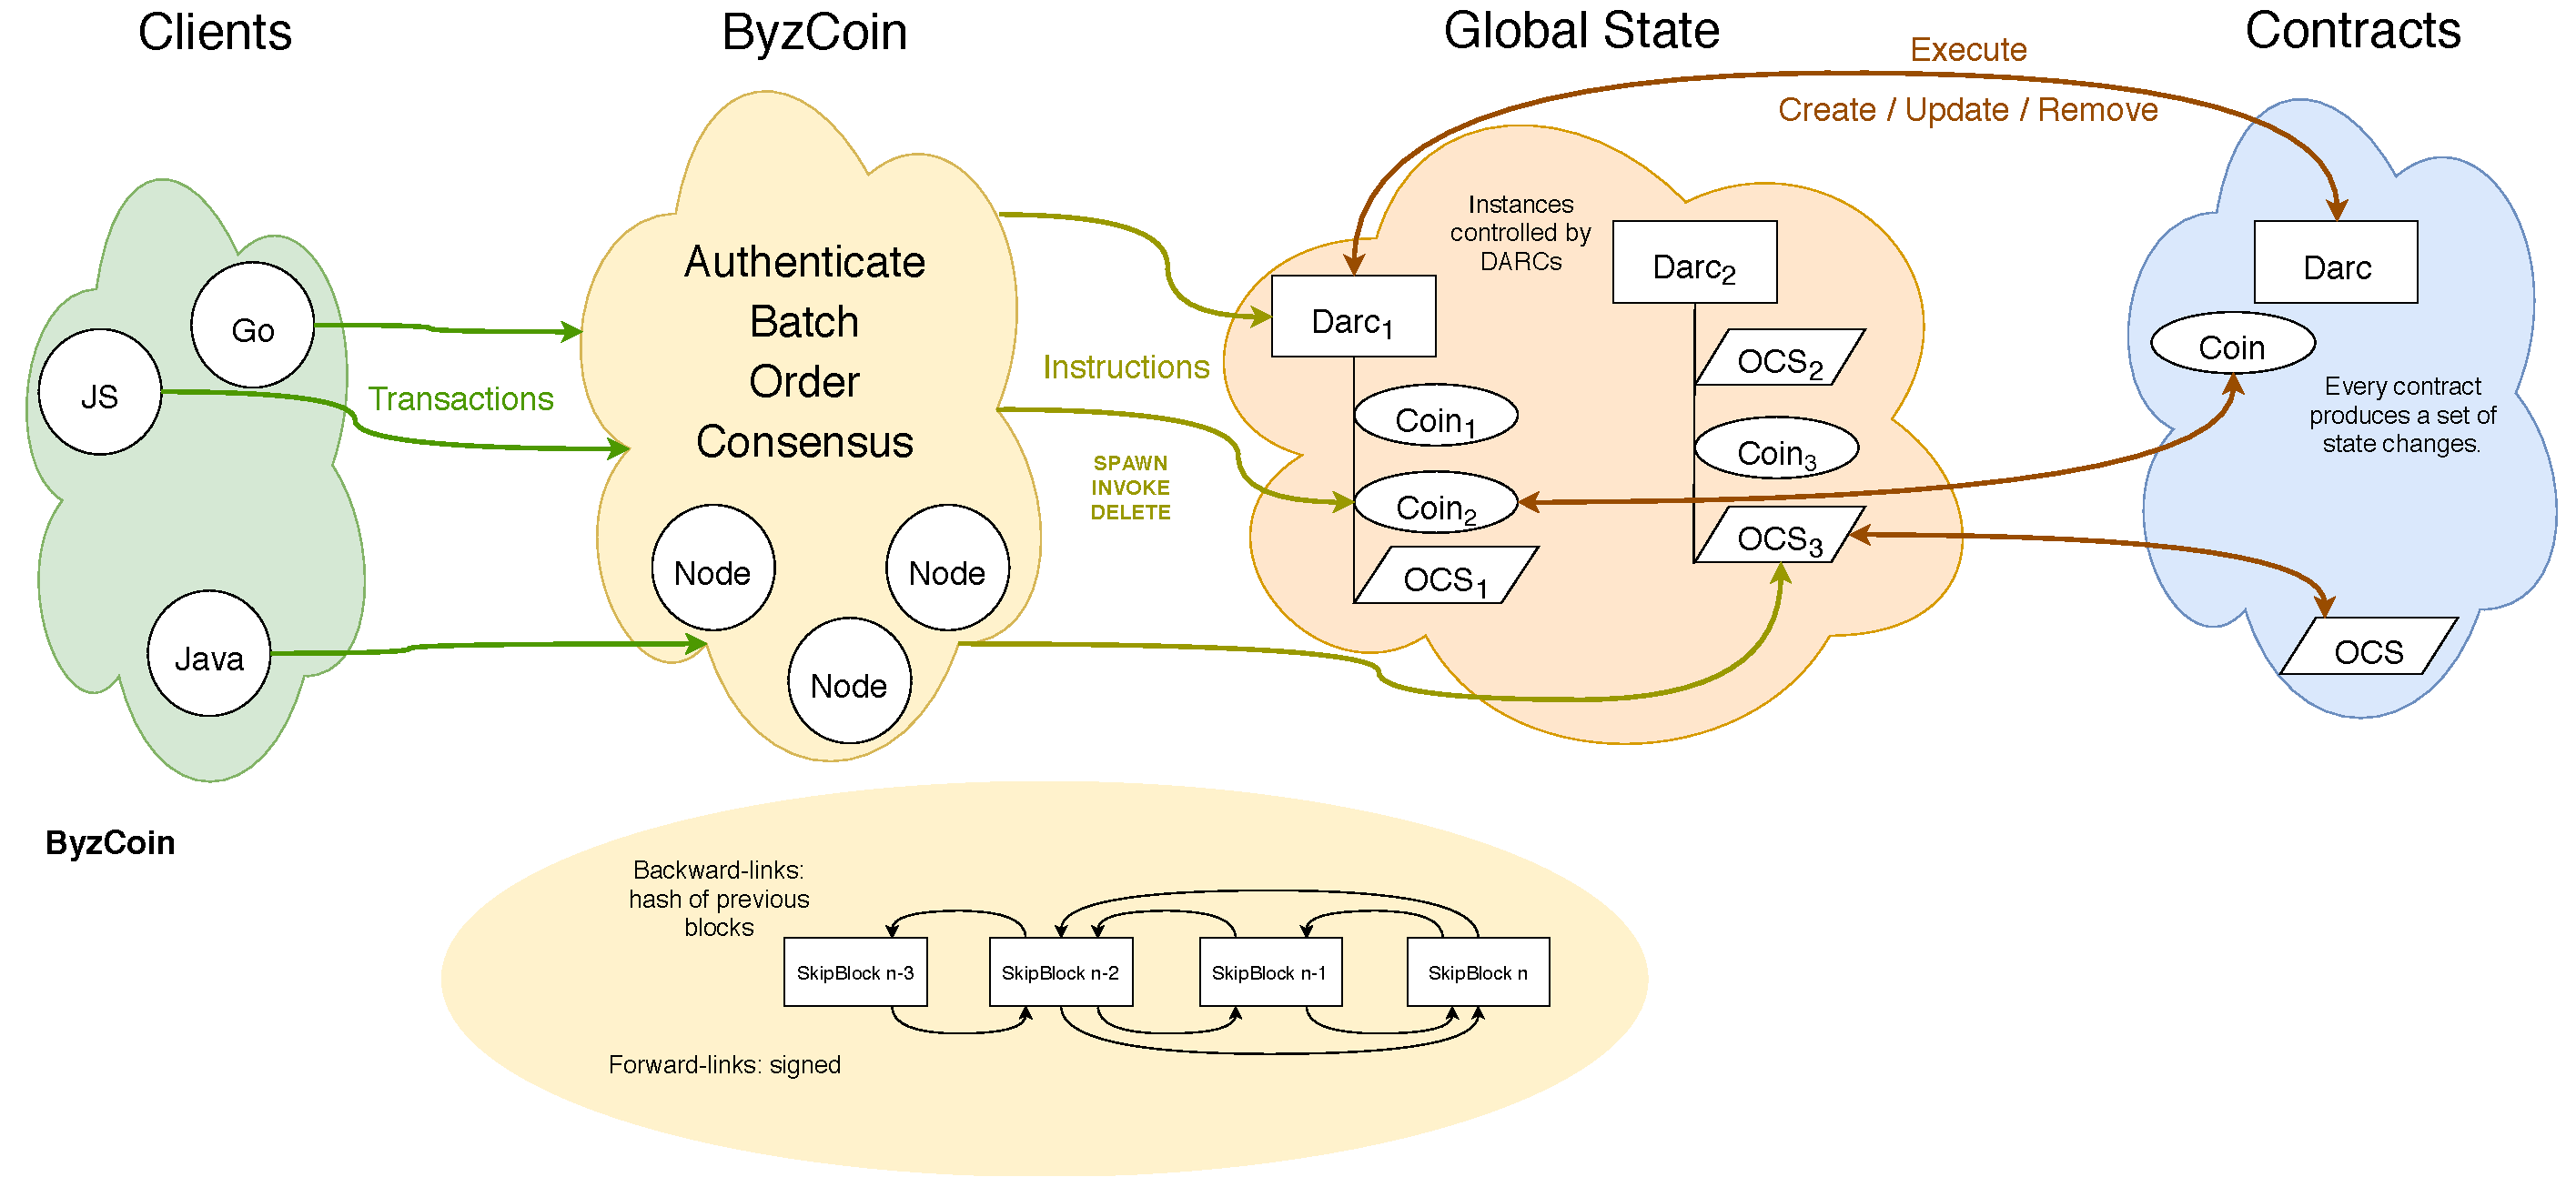
\includegraphics[width=1\textwidth]{Figures/ByzCoin.pdf}
    \caption{ByzCoin (Simplified version of \cite{ByzCoin Figure})}
    \label{ByzCoin}
\end{figure}
\noindent
Instead of using a standard chain of blocks, where only neighbors are connected, the DEDIS team presents a data structure that combines
blockchains and skip-lists \cite{SkipLists} and names it a \textbf{skipchain} \cite{Chainiac}.\\
\newline
Skipchains enable both backward and forward timeline traversal with single or multi-hop links. The backward links are cryptographic hashes of past blocks and the forward links are cryptographic signatures of future blocks that are added retroactively when the target block appears \cite{Chainiac}. These forward links allow future block validation, which is especially useful in scenarios such as software updates, where an outdated client gets an update from a not necessarily trusted peer \cite{Chainiac}.
\newline
The long-distance links allow traversal in a lower number of steps (logarithmic cost) and provide shorter proofs of existence. ByzCoin is, so far, the only blockchain technology that uses this concept in order to prove that a given instance exists without having to know the whole blockchain. Skipchains also enable clients to verify that transactions are on the blockchain without the need of being connected to the Internet \cite{Chainiac}.\\
\newline
Another clear benefit that ByzCoin \cite{ByzCoin} blockchain provides is management of the access policies in the system in a dynamic and fully decentralized manner. As a substitute for a password or public key for authentication, a DARC (Distrubuted Access Right Control) structure is being used \cite{Darc}. It allows evolution of the description about who can or cannot access a certain resource, by maintaining a set of changeable rules. How these DARC structures are implemented is explained in details in section~\ref{DARCs}.\\
\newline
Taking into consideration that most of the existing blockchain applications which contain sensitive and private data use either semi centralized approaches (secret data is not stored on the chain) \cite{Medical Data, Calypso} or ignore the privacy problem \cite{Privacy, Calypso}, the DEDIS Laboratory introduces a framework called Calypso \cite{Calypso}. Calypso provides a secure way of sharing confidential data over a blockchain and also prevents a single point of compromise or failure in the system by
keeping the private data as on-chain secrets (using threshold cryptography) \cite{Calypso}.\\
\newline
The primary goal of Calypso is to allow only authorized clients to decrypt the on-chain secrets, while maintaining at the same time a tamper-resistant log of every access transaction \cite{Calypso}.\\
\newline
The overview of the Calypso framework architecture is shown in Figure~\ref{Calypso Overview}. It involves a writer, a reader and two collective authorities (groups of signers) \cite{CoSi}.
\newline
The first one is called \textbf{access control cothority} and is responsible for verifying and logging write and read transactions, as well as enforcing access control policies. It consists of the same conodes that run the ByzCoin blockchain protocol, but these servers also have the Calypso read and write contracts compiled in their binaries.
\newline
The second one is named a \textbf{secret-management cothority} and is in charge of handling and delivering secrets.\\
\newline
The process of storing and reading on-chain secrets goes as follows:
\newline
\begin{enumerate}[start=0]
    \item Initially, an administrator generates collective private-public key pair for the secret-management cothority, by running a Distributed Key Generation algorithm.
    \item The writer creates a symmetric key to encrypt his/her secret and then encrypts this symmetric key with the collective public key of the secret-management cothority \cite{Calypso}.
    \item The encrypted secret and its access policy are stored on the blockchain and a reader is able to download the secret and request to read it. The read request is verified by the secret-management cothority and then logged on the blockchain.
    \item The reader uses the logged read request to ask the secret-management cothority to re-encrypt the initial symmetric key with his/her public key.
    \item  The reader can decrypt the symmetric key and therefore decode the secret.
\end{enumerate}
Providing a secure sharing of sensitive data with dynamic management of access policies and ownership, is what makes Calypso and the ByzCoin blockchain a perfect match for our project.\\
\newline
Car owners are able to grant access to their car service history to potential buyers in order to increase the value (price) of the car, with the possibility to remove the access if the buyer is no longer interested.
Additionally, every read and write transaction is logged and the history of the system cannot be compromised if less than $\frac{1}{3}$ of malicious nodes are present.

\begin{figure}[H]
    \centering
    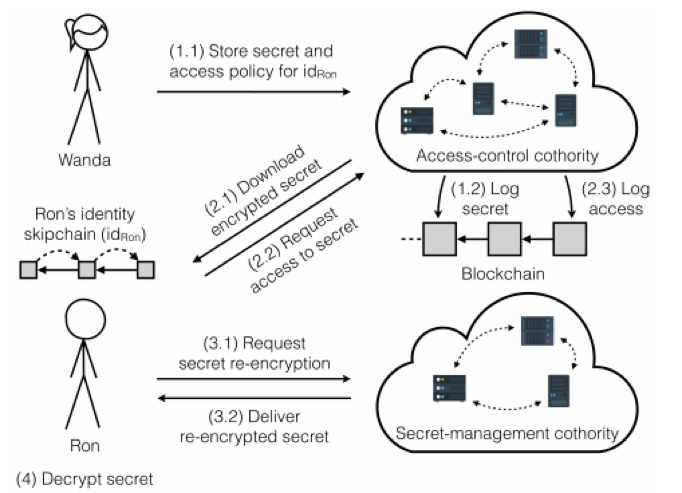
\includegraphics{Figures/Calypso.png}
    \caption{Calypso Overview \cite{Calypso}}
    \label{Calypso Overview}
\end{figure}

